\documentclass[12pt]{article}
\usepackage{array}
\usepackage{amsmath}
\usepackage{mathtools}
\usepackage{gensymb}
\usepackage{graphicx}
\usepackage{float}

\setlength{\parindent}{1cm}
\allowdisplaybreaks

\begin{document}
    \title{Acceleration due to Gravity and the Coefficient of Kinetic Friction of an Air Track and Cart.}
    \author{Ryan Coyne and Patrick Browning}
    \maketitle
    \section{Abstract}

        \paragraph{} The acceleration due to gravity, $g$, and the coefficient 
        of kinetic friction, $\mu$, of an air track and cart were
         measured using a meter stick, and a sound based motion sensor. 
        $g$ was measured to be (\(11.20 \pm 0.23\)) \(\frac{\text{m}}{\text{s}^2}\) and $\mu$ was measured to be 
        (\(0.00268 \pm 0.00061\)).
    \section{Introduction}
    \paragraph{}This experiment measured the acceleration due to gravity and a coefficient of kinetic friction. Acceleration is a measurement of how a velocity changes with time.
       This specific acceleration is caused by the force of gravity exerted by all matter but in this case is primarily dependant on the mass and radius of Earth. The 
       coefficient of kinetic friction is a scalar value with no units that is multiplied by the normal force to find the force of friction between two objects when they are 
       touching and in motion relative to one another. The force of kinetic friction is always in the opposite direction of the motion of the object it is acting upon and 
       has the same magnitude as long as the normal force is the same, therefore the acceleration due to that friction has the same properties. The acceleration due to gravity 
       is always in a consistent direction regardless of the motion of the object being accelerated by gravity.
       \paragraph{} These properties can be used to create a system of equations which allow us to solve for each of these values, gravity, $g$, and the coefficient of kinetic 
       friction, $\mu$. Let us say that an object is moving in one direction under only the influence of gravity and friction and it's acceleration is measured and then moves in the opposite 
       direction under the same conditions and it's acceleration is measured for this direction as well. We can then create an equation that describes the net acceleration 
       of the object where both equations are only dependant on \(g\) and \(\mu\). We now have a system two equations that are not equivalent and are dependant on two variables. 
       These equations meet the conditions under which we can solve a system of equations and by doing so can find the values for \(g\) and \(\mu\).
    \section{Procedure}
    \paragraph{}The length of an air track and the height of a wooden block were measured using a meter stick. The air track
        and wooden block were placed on a table with one side of the air track propped up on the wooden block. A sound based
        motion detector was placed at the higher end of the track and was pointed down the track. A cart with a metal sail was placed at the top of the track and 
        was released to slide down the track as the motion sensor tracked it's movement. This was repeated five times. The cart was then placed at the bottom of the 
        track and given a sharp push up the track so that the cart was only being pushed for a short time. This was repeated five times. Lastly a quadratic fit was applied 
        to each of the sets of position data acquired from the motion sensors to find an approximate equation for the position which was used to find the acceleration.
        \begin{figure}[h]
            \caption{Experimental Setup}
            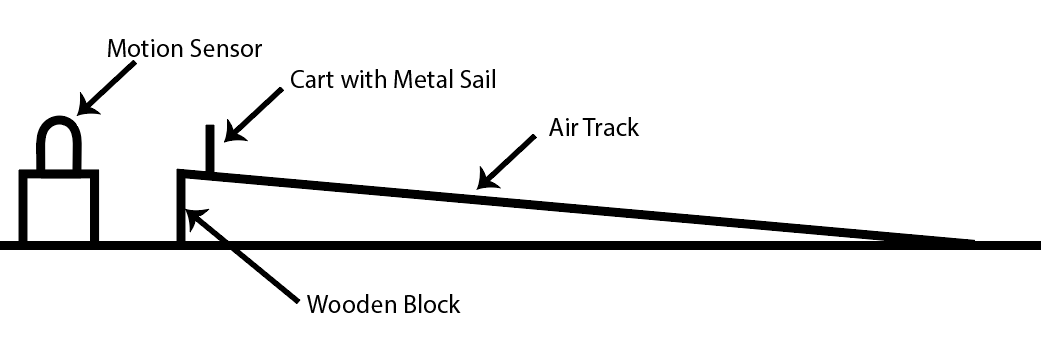
\includegraphics[width=\linewidth]{Figure 1 - Experiment Setup.png}
            \label{fig:setup}
        \end{figure}
    \section{Data}
        \begin{center}
            \begin{tabular} {>{\centering\arraybackslash}p{0.07\textwidth}|>{\centering\arraybackslash}p{0.1\textwidth}>{\centering\arraybackslash}p{0.1\textwidth}|>{\centering\arraybackslash}p{0.1\textwidth}>{\centering\arraybackslash}p{0.1\textwidth}>{\centering\arraybackslash}p{0.1\textwidth}|}
                \multicolumn{5}{c}{Table 1. Determining g and $\mu$}\\ 
                Trial & $h(\text{cm})$ & $l(\text{cm})$ & $a_u(\frac{\text{m}}{\text{s}^2})$ & $a_d(\frac{\text{m}}{\text{s}^2})$\\ 
                \hline
                1 & 3.29 & 99.99 & 0.422 & 0.340\\
                2 & 3.21 & 99.98 & 0.404 & 0.340\\
                3 & 3.30 & 100.05 & 0.398 & 0.336\\
                4 & 3.28 & 100.01 & 0.384 & 0.340\\
                5 & 3.31 & 100.03 & 0.388 & 0.340\\
                \hline
                $\overline{x}$ & 3.298 & 100.012 & 0.3992 & 0.3392\\
                \(\sigma\) & 0.013 & 0.029 & 0.015 & 0.018\\
            \end{tabular}\\[12pt]
            \begin{tabular}{c|c|c}
                \multicolumn{3}{c}{Table 2. Results}\\
                 & $g \frac{\text{m}}{\text{s}^2}$ & $\mu$\\
                 \hline
                 \(\overline{x}\) & 11.20 & 0.00268\\
                 \(\sigma\) & 0.23 & 0.00061
            \end{tabular}
            \begin{figure}[H]
                \caption{Position vs. Time with Fit}
                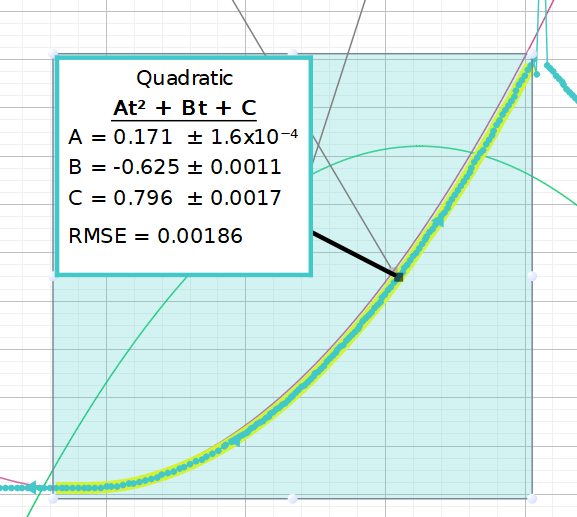
\includegraphics[width=\linewidth]{Figure 2 - Position and Fit.png}
            \end{figure}
        \end{center}

    \section{Calculations}
        \begin{align}
            a_d &= g sin \theta - \mu g cos \theta \nonumber\\
            a_u &= g sin \theta + \mu g cos \theta \nonumber \\
            a_u + a_d &= 2 g sin \theta \\
            g &= \frac{a_u + a_d}{2 sin \theta} \nonumber\\
            a_u - a_d &= 2 \mu g cos \theta \\
            a_u - a_d &= 2 \mu (\frac{a_u + a_d}{2 g sin \theta}) cos \theta \nonumber \\
            a_u - a_d &= \mu (a_u + a_d) cot \theta \nonumber\\
            \mu &= \frac{a_u - a_d}{a_u +a_d} tan \theta \nonumber\\
            \overline{h} &= \frac{3.29\text{cm}+3.31\text{cm}+3.30\text{cm}+3.28\text{cm}+3.31\text{cm}}{5}\\
            &= \frac{16.49\text{cm}}{5} \nonumber\\
            &= 3.2\underline{9}8 \text{cm}\nonumber\\
            \sigma_h^2 &= \frac{1}{4} \sum_{i=1}^5 (h_i - \overline{h})^2\\
            A_h &= (3.29\text{cm}-3.298\text{cm})^2 \nonumber \\
            B_h &= (3.31\text{cm}-3.298\text{cm})^2 \nonumber \\
            D_h &= (3.3\text{cm}-3.3298\text{cm})^2 \nonumber \\
            E_h &= (3.29\text{cm}-3.3298\text{cm})^2 \nonumber \\
            F_h &= (3.31\text{cm}-3.298\text{cm})^2 \nonumber \\
            \sigma_h^2 &= \frac{A_h + B_h + D_h + E_h + F_h }{4}\nonumber\\
            &= \frac{0.000676\text{cm}^2}{4}\nonumber\\
            &=0.000169\text{cm}^2\nonumber\\
            \sigma_h &= \sqrt{0.000169\text{cm}^2} \nonumber\\
            &=0.013\text{cm} \nonumber \\
            \delta_h &= \frac{0.013\text{cm}}{3.298\text{cm}} \\
            &= 0.3\underline{9}53 \% \nonumber \\
            \delta_l &= \frac{0.029\text{cm}}{100.012\text{cm}} \nonumber \\
            &= 0.02\underline{8}6\% \nonumber \\
            \delta_{au} &= \frac{0.015\text{cm}}{0.3992\text{cm}} \nonumber \\
            &= 3.7\underline{5}9 \% \nonumber \\ 
            \delta_{ad} &= \frac{0.018\text{cm}}{0.3392\text{cm}} \nonumber \\
            &= 0.5\underline{2}7 \% \nonumber \\
            \theta &= sin^{-1}\frac{\overline{h}}{\overline{l}}\\
            &= sin^{-1}\frac{3.298 \text{cm}}{100.012 \text{cm}}\nonumber \\
            & = 1.88\underline{9}73 \degree \nonumber \\
            \overline{g} &= \frac{0.3392 \frac{\text{m}}{\text{s}^2} + 0.3992 \frac{\text{m}}{\text{s}^2}}{2 sin(1.88973 \degree)} \\
            &= 11.\underline{1}96 \frac{\text{m}}{\text{s}^2}\\
            g_{d} &= \frac{0.3392\frac{\text{m}}{\text{s}^2} + 0.0018 \frac{\text{m}}{\text{s}^2} + 0.3992 \frac{\text{m}}{\text{s}^2}}{2 sin(1.88973 \degree)}\nonumber\\
            &= 11.\underline{2}2313 \frac{\text{m}}{\text{s}^2 }\nonumber \\
            g_u &= \frac{0.3392\frac{\text{m}}{\text{s}^2} + 0.015 \frac{\text{m}}{\text{s}^2} + 0.3992 \frac{\text{m}}{\text{s}^2}}{2 sin(1.88973 \degree)}\nonumber \\
            &= 11.\underline{4}2355 \frac{\text{m}}{\text{s}^2 }\nonumber\\
            \sigma^2_g &= (11.22313\frac{\text{m}}{\text{s}^2 } - 11.196\frac{\text{m}}{\text{s}^2 })^2 + (11.42355\frac{\text{m}}{\text{s}^2 } - 11.196\frac{\text{m}}{\text{s}^2 })^2 \nonumber \\
            &= 0.05251(\frac{\text{m}}{\text{s}^2 })^2\nonumber\\
            \sigma_g &= \sqrt{0.05251} \frac{\text{m}}{\text{s}^2 }\nonumber\\
            &= 0.23 \frac{\text{m}}{\text{s}^2 }\nonumber \\
            \overline{\mu} &= \frac{0.3992 \frac{\text{m}}{\text{s}^2} - 0.3392\frac{\text{m}}{\text{s}^2 }}{0.3992\frac{\text{m}}{\text{s}^2 }+0.3392\frac{\text{m}}{\text{s}^2 }}tan(1.88973\degree)\\
            &= 0.0026\underline{8}1 \nonumber\\
            \mu_d &= \frac{0.3992\frac{\text{m}}{\text{s}^2 } + 0.00789\frac{\text{m}}{\text{s}^2 } - 0.3392\frac{\text{m}}{\text{s}^2 }}{0.3992\frac{\text{m}}{\text{s}^2 } + 0.001789\frac{\text{m}}{\text{s}^2 } +0.3392\frac{\text{m}}{\text{s}^2 }}tan(1.88973\degree)\\
            &= 0.0025\underline{9}5\nonumber\\
            \mu_u &= \frac{0.3992\frac{\text{m}}{\text{s}^2 } - 0.015007\frac{\text{m}}{\text{s}^2 } - 0.3392\frac{\text{m}}{\text{s}^2 }}{0.3992\frac{\text{m}}{\text{s}^2 } + 0.015007\frac{\text{m}}{\text{s}^2 } +0.3392\frac{\text{m}}{\text{s}^2 }}tan(1.88973\degree)\nonumber\\
            &= 0.0032\underline{8}5\nonumber\\
            \sigma^2_{\mu} &= (0.002595-0.002681)^2+(0.003285-0.002681)^2\nonumber\\
            &= 3.71992x10^{-7}\nonumber\\
            \sigma_{\mu} &= \sqrt{3.71992x10^{-7}}\nonumber\\
            &= 0.00061\nonumber
        \end{align}
    \section{Conclusion}
    \paragraph{}We measured $g$ to be (\(11.20 \pm 0.23\)) \(\frac{\text{m}}{\text{s}^2}\) and $\mu$ to be 
        (\(0.00268 \pm 0.00061\)). $g$ is expected to be within two standard deviations of $9.8$ \(\frac{\text{m}}{\text{s}^2}\)
        and $\mu$ was expected to be within 0. A potential cause of this deviation from the expected values is the table or 
        floor may have been at an angle that was not taken into consideration. Another possible contribution to the deviation
         is that the height of the block was irregular and so what we measured may have been slightly different from the 
        actual height of the block. Either of these could have caused the angle between the air track and the plane perpendicular to 
        the force of gravity to be greater than the angle that was measured, which could have in turn caused our results to be higher 
        than expected. Our professor also instructed us to neglect the error on $h$ even though it's  relative error was greater than 
        ten percent of the highest relative error. 
\end{document}